\begin{frame}{Metrics}
\begin{itemize}
\item Expected Gain  --- (Nugget Precision) 
 average number of novel nuggets matched to each update

\vspace{10pt}
\item Comprehensiveness --- (Nugget Recall) percent of unique nuggets matched
by update summary
\vspace{10pt}
\item F1 --- Harmonic Mean of Expected Gain and Comprehensiveness

\vspace{10pt}
\item Latency Weighted variants of the above metrics
\begin{itemize}
\item Value of each nugget match decreases to 0 if it is extracted after its reference time.
\item Value of each nugget match increases to as much as 2 if it is 
extracted before its reference time.
\end{itemize}

\end{itemize}


\end{frame}


\begin{frame}{Evaluations}

\begin{itemize}
\item Temporal Summarization Shared-Tasks at TREC 2014 
\begin{itemize}
\item Submitted SAP.
\end{itemize}
\item Temporal Summarization Shared-Tasks at TREC 2015
\begin{itemize}
\item Submitted L2S, and SAP.
\end{itemize}
\vspace{10pt}
\item Performed our own automatic $k$-fold evaluations of SAP and L2S summarizers. 
\end{itemize}
\end{frame}

\begin{frame}{TREC 2014 Evaluation}
\begin{columns}
\begin{column}{0.5\textwidth}
\begin{itemize}
\item SAP was \textbf{first} in overall metric, latency weighted F1 
\vspace{10pt}
\item SAP increases Expected Gain over AP-Clustering only baseline.
\vspace{10pt}
\item SAP had \begin{itemize}
\item above average Expected Gain, 
\item slightly below average Comprehensiveness, 
\item better latency than the top 3 highest Expected Gain runs, 
\end{itemize}
\end{itemize}
\end{column}
\begin{column}{0.5\textwidth}
\begin{tikzpicture}
\node at (0,0) {\resizebox{0.70\textwidth}{!}{
\begin{tabular}{cccccc}
\toprule
TeamID & RunID &Exp. Gain & Comp. & Comp. (Latency) & F1 (Latency) \\
\midrule
\textbf{cunlp} & \textbf{2SAP} & 0.0631 & 0.3220 & 1.2068 & \textbf{0.1162} \\
BJUT & Q1 & \textbf{0.0657} & 0.4088 & 1.1491 & 0.1110\\
BJUT & Q2 & 0.0632 & 0.3979 & 1.1669 & 0.1091\\
BJUT & Q0 & 0.0632 & 0.3979 & 1.1669 & 0.1091\\
uogTr & uogTr2A & 0.0467 & 0.4453 & 1.2322 & 0.0986\\
uogTr & uogTr4AC & 0.0347 & 0.4539 & 1.2751 & 0.0793\\
uogTr & uogTr4ARas & 0.0387 & 0.3691 & 1.2328 & 0.0772\\
IRIT & KW30H5NW3600 & 0.0383 & 0.3521 & 1.2221 & 0.0723\\
IRIT & KW30H5NW300 & 0.0378 & 0.3538 & 1.2208 & 0.0714\\
uogTr & uogTr4A & 0.0281 & \textbf{0.4733} & 1.2522 & 0.0677\\
\midrule
\multicolumn{2}{c}{\textit{average}} & 0.0327 & 0.3615 & 1.2943 & 0.0620\\
\midrule
IRIT & KW80H5NW3600 & 0.0289 & 0.3764 & 1.2191 & 0.0604\\
IRIT & KW30H10NW300 & 0.0298 & 0.3780 & 1.2617 & 0.0602\\
cunlp & 1APSalRed & 0.0325 & 0.3058 & 1.1507 & 0.0602\\
IRIT & KW80H5NW300 & 0.0285 & 0.3806 & 1.2164 & 0.0596\\
ICTNET & run3 & 0.0531 & 0.1081 & 0.7004 & 0.0530\\
BUPT\_PRIS & Cluster4 & 0.0155 & 0.2692 & 1.9140 & 0.0508\\
IRIT & KW80H10NW300 & 0.0225 & 0.4012 & 1.2621 & 0.0503\\
BUPT\_PRIS & Cluster3 & 0.0115 & 0.3380 & 1.9165 & 0.0407\\
\textbf{cunlp} & \textbf{3AP} & 0.0174 & 0.4265 & 1.3689 & 0.0403\\
ICTNET & run2 & 0.0418 & 0.0934 & 0.6266 & 0.0311\\
BUPT\_PRIS & Cluster2 & 0.0059 & 0.3728 & 1.9170 & 0.0222\\
ICTNET & run4 & 0.0079 & 0.4070 & 1.2364 & 0.0178\\
ICTNET & run1 & 0.0070 & 0.4090 & 1.2314 & 0.0160\\
BUPT\_PRIS & Cluster1 & 0.0033 & 0.4369 & \textbf{1.9175} & 0.0127\\
\bottomrule
\end{tabular}}};
\node (e2) at (-2.25,2.05) {};
\node (s2) at (-3,2.05) {};
\node (e1) at (-2.25,-1.4) {};
\node (s1) at (-3,-1.4) {};
\draw[line width=0.7mm,->] (s1) -- (e1);
\draw[line width=0.7mm,->] (s2) -- (e2);
\node  at ($(s1.north)!0.5!(e1.north)+(0,0.15)$) {\large \textbf{AP}};
\node  at ($(s2.north)!0.5!(e2.north)+(0,0.15)$) {\large \textbf{SAP}};
\end{tikzpicture}
\end{column}
\end{columns}

\end{frame}

\begin{frame}{Automatic \textsc{Rouge} Evaluation}
\begin{columns}
\begin{column}{0.5\textwidth}
    \begin{tikzpicture}
        \node at (0,0) {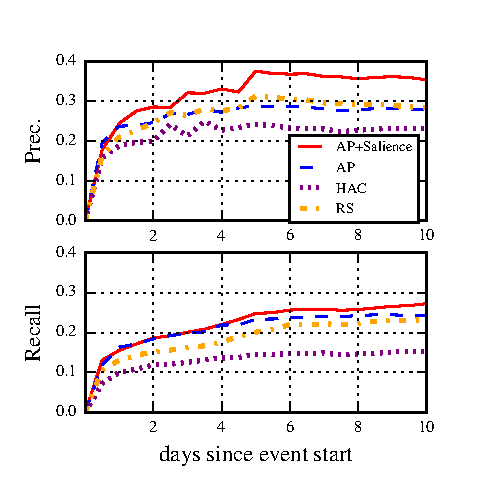
\includegraphics[]{images/strm/rouge-time.eps}};
        \node[draw=white,fill=white,text width=1.05cm] at (2.20,1.55) {};
        \node[draw=white,fill=white,inner sep=0pt,text width=1.05cm] at (2.20,1.60) {\tiny SAP};
        \node[draw=white,fill=white,text width=1.05cm] at (2.20,1.30) {};
        \node[draw=white,fill=white,text width=1.05cm] at (2.20,0.95) {};
        \node[draw=white,fill=white,text width=1.05cm] at (2.20,0.55) {};

        \node[draw=white,fill=white,inner sep=0pt,text width=1.05cm] at (2.20,1.25) {\tiny AP};
        \node[draw=white,fill=white,inner sep=0pt,text width=1.05cm] at (2.20,0.90) {\tiny HAC};
        \node[draw=white,fill=white,inner sep=0pt,text width=1.05cm] at (2.20,0.55) {\tiny RS};
    \end{tikzpicture}
\end{column}
\begin{column}{0.5\textwidth}
\begin{itemize}
\item SAP achieves higher \textsc{Rouge}-1 precision faster than baselines
\vspace{10pt}

\end{itemize}
\end{column}
\end{columns}

\end{frame}


\begin{frame}{Automatic Rouge Evaluation}
    \begin{columns}
        \begin{column}{0.5\textwidth}
            \begin{center}
    \begin{tabular}{l c c }
            \toprule
        Model & \multicolumn{2}{c}{\textsc{Rouge}-1 F1} \\
                \midrule
        Full System & 0.306 \\
                \midrule
                No Simple  &  0.294 & \small (-.012)\\ 
                No Query &  0.280 & \alert<1>{\small (-.026)}\\ 
                No Geo   &  0.265 &\alert<1>{\small (-.041)}\\ 
                No LM     &  0.254 &\alert<1,2>{\small (-.052)}\\
                \midrule
                AP only  &  0.263 & \alert<2>{\small (-.043)} \\
                \bottomrule
            \end{tabular}
            \end{center}
        \end{column}
        \begin{column}{0.5\textwidth}
            
            \begin{itemize}
                \item Content features are more important than heuristics like position.

                \item<2-> Removing LM is worse than having no salience estimation.

            \end{itemize}

        \end{column}
    \end{columns}

\end{frame}


\begin{frame}{TREC 2015 Evaluation}
\begin{columns}
\begin{column}{0.5\textwidth}
\begin{itemize}
    \item L2S was \textbf{4th and 5th}, SAP was \textbf{7th} in overall metric, latency weighted F1 
\vspace{10pt}
\item L2S and SAP runs above average
\vspace{10pt}
\item L2S improves over SAP on all metrics
\end{itemize}
\end{column}
\begin{column}{0.5\textwidth}
\begin{tikzpicture}
\node at (0,0) {\resizebox{0.90\textwidth}{!}{
\begin{tabular}{cccccc}
\toprule
Team ID & Run ID & Expected Gain & Comp. & Comp. (Latency) & F1 (Latency) \\
\midrule
WaterlooClarke & UWCTSRun1 & 0.2350 & 0.3520 & 0.6612 & \textbf{0.1762}\\
WaterlooClarke & UWCTSRun3 & 0.2252 & 0.3421 & \textbf{0.6643} & 0.1718\\
WaterlooClarke & UWCTSRun2 & \textbf{0.2872} & 0.2584 & 0.6551 & 0.1710\\
\textbf{cunlp} & \textbf{3LtoSfltr5} & 0.1371 & 0.4870 & 0.6392 & 0.1282\\
\textbf{cunlp} & \textbf{1LtoSfltr20} & 0.1203 & 0.5372 & 0.6287 & 0.1100\\
IRIT & FS1A & 0.0849 & 0.4959 & 0.6051 & 0.0719\\
\textbf{cunlp} & \textbf{4SAP} & 0.1011 & 0.4584 & 0.5108 & 0.0674\\
\midrule
\multicolumn{2}{c}{\textit{average}} & 0.0666 & 0.4342 & 0.4697 & 0.0499\\
\midrule
IRIT & FS2A & 0.0518 & 0.5899 & 0.6285 & 0.0476\\
BJUT & DMSL1NMF2 & 0.0445 & 0.6123 & 0.4539 & 0.0354\\
BJUT & DMSL1AP1 & 0.0413 & \textbf{0.6155} & 0.4701 & 0.0338\\
l3sattrec15 & l3sattrec15run1 & 0.0408 & 0.3612 & 0.3743 & 0.0268\\
l3sattrec15 & l3sattrec15run3 & 0.0400 & 0.3669 & 0.3712 & 0.0262\\
IRIT & FS1B & 0.0422 & 0.2939 & 0.3913 & 0.0259\\
IRIT & FS2B & 0.0306 & 0.3391 & 0.4491 & 0.0239\\
USI & InL2DecrQE1ID1 & 0.0182 & 0.5713 & 0.5806 & 0.0196\\
USI & InL2DecrQE2ID2 & 0.0169 & 0.5758 & 0.5836 & 0.0184\\
udel\_fang & WikiOnlyFS2 & 0.0206 & 0.5819 & 0.4600 & 0.0176\\
udel\_fang & ProfOnlyFS3 & 0.0258 & 0.5294 & 0.4122 & 0.0174\\
USI & InL2StabQE2ID3 & 0.0171 & 0.6133 & 0.5238 & 0.0170\\
udel\_fang & WikiProfMixFS1 & 0.0189 & 0.5965 & 0.4660 & 0.0166\\
l3sattrec15 & l3sattrec15run2 & 0.0283 & 0.2276 & 0.2560 & 0.0164\\
USI & InL2IncrQE2ID4 & 0.0179 & 0.5837 & 0.2888 & 0.0108\\
\bottomrule
\end{tabular}}
};
\node (e2) at (-3.0,1.65) {};
\node (s2) at (-3.75,1.65) {};
\node (e1) at (-3.00,0.95) {};
\node (s1) at (-3.75,0.95) {};
\draw[line width=0.7mm,->] (s1) -- (e1);
\draw[line width=0.7mm,->] (s2) -- (e2);
\node  at ($(s1.north)!0.5!(e1.north)+(0,0.15)$) {\large \textbf{SAP}};
\node  at ($(s2.north)!0.5!(e2.north)+(0,0.15)$) {\large \textbf{L2S}};
\end{tikzpicture}
\end{column}
\end{columns}

\end{frame}


\begin{frame}{Automatic Evaluation}
    \begin{center}
\resizebox{0.5\textwidth}{!}{
\begin{tabular}{ l   c  c }
\toprule
%   &\multicolumn{3}{c}{unpenalized}&\multicolumn{3}{c}{latency-penalized}&\\
% \cmidrule(lr){2-4} \cmidrule(lr){5-7}
%   &
Model  & Nugget  F1 & Nugget F1 (latency) \\ % & Num. Updates \\
    \midrule
%\textsc{AP}         
%    & $0.083$            & $0.09$                     & $0.078$ 
%    & $0.079$            & $0.095$                    & $0.077$ 
%    & ~~$20.846$ \\
\textsc{SAP}      
& $0.094$ & \alert<2>{$0.088$} \\
   % & ~~~~$8.333$ \\
%\textsc{Cos}     
 %   & $0.075$            & $0.176$              & $0.099$ 
 %   & $0.095$            & $0.236$              & $0.128$ 
 %   & $145.615$ \\
\textsc{L2S}    &  ${\bf0.112}$  & \alert<3>{${\bf0.162}$} \\
   % & ~~$89.872$ \\
%\textsc{L2S-Cos}
%    & $0.115$        & $0.189$ & ${\bf0.127}$
%    & ${\bf0.162}$ & $0.276$ & ${\bf0.184}$
% & ~~$29.231$ \\
\bottomrule
\end{tabular}}
\end{center}

%\resizebox{\textwidth}{!}{
%\begin{tabular}{ l   c c c   c c c  c }
%\toprule
%   &\multicolumn{3}{c}{unpenalized}&\multicolumn{3}{c}{latency-penalized}&\\
% \cmidrule(lr){2-4} \cmidrule(lr){5-7}
%   & Exp. Gain     & Comp. 
%        & F1 & Exp. Gain     & Comp& F1 \\ % & Num. Updates \\
%    \bottomrule
%%\textsc{AP}         
%%    & $0.083$            & $0.09$                     & $0.078$ 
%%    & $0.079$            & $0.095$                    & $0.077$ 
%%    & ~~$20.846$ \\
%\textsc{SAP}      
%    & \alert<2>{$\mathbf{0.119}$} & $0.09$                     & $0.094$ 
%    & $0.105$            & $0.088$                    & $0.088$ \\
%   % & ~~~~$8.333$ \\
%%\textsc{Cos}     
% %   & $0.075$            & $0.176$              & $0.099$ 
% %   & $0.095$            & $0.236$              & $0.128$ 
% %   & $145.615$ \\
%\textsc{L2S}       
%    & $0.097$            & \alert<3>{$\mathbf{0.207}$}   & \alert<3>{${\bf0.112}$ }
%    & \alert<4>{${\bf0.136}$}      & \alert<4>{$\mathbf{0.306}$} & \alert<4>{${\bf0.162}$} \\
%   % & ~~$89.872$ \\
%%\textsc{L2S-Cos}
%%    & $0.115$        & $0.189$ & ${\bf0.127}$
%%    & ${\bf0.162}$ & $0.276$ & ${\bf0.184}$
%% & ~~$29.231$ \\
%\bottomrule
%\end{tabular}}}

\begin{itemize}
\item<2-> SAP was retrieving nuggets after the reference time, getting a latency penalty.
\item<3-> L2S beat reference times, getting a latency reward!

\end{itemize}
\end{frame}

\begin{frame}{L2S and Position Heuristics}

\begin{center}
  \begin{tabular}{ l   c c c  }
\toprule
    &\multicolumn{3}{c}{latency-penalized}\\
\cmidrule(lr){2-4}
    & Exp. Gain    & Comp. & F1 \\
    \midrule
  %  \textsc{Cos}  & $0.095$ & $\mathbf{0.236}$ & $0.128$ \\
     \textsc{L2S}  & $0.136$ & \alert{$0.306$} & $0.162$ \\
     \textsc{L2S-FS}  & $0.164$ & \alert{$0.220$} & $0.157$ \\
%    \textsc{L2S-Cos-FS} &
 %     $\mathbf{0.207}$ & $0.18~~$ & $\mathbf{0.163}$ \\
\bottomrule
  \end{tabular}
\end{center}

\begin{itemize}
\item L2S-FS (limited to first sentences) misses out on information in the body
\item<2> A good content model of salience is neccessary to find information in the body.
\end{itemize}


\end{frame}

\begin{frame}{Takeaways}

 We proposed two summarization models for query focused, news-stream summarization.
\begin{itemize}
                    \item SAP model -- Combines salience estimation + AP clustering.
\vspace{5pt}

                    \item L2S model -- greedy online summarizer, identifies salient information more quicly than SAP/baselines.

\vspace{5pt}
                    \item We denomstrate the importance of content features 
when modeling salience in this environment.
                \end{itemize}




\end{frame}
